\section{Method}
\label{sec:method}

In this section, we detail our workflow\footnote{The code and a live demo are available at \url{https://anonymous.4open.science/r/Dog_Script-CDB0}}(\figref{fig:Workflow}) including audio clean-up by AudioSep, sentence extracting, phoneme recognition, phoneme combination, and word discovery. 
% Implementation details can be found in Appendix~\ref{sec:appendix_a}.

\begin{figure}[th]
    \centering
    \scalebox{0.35}{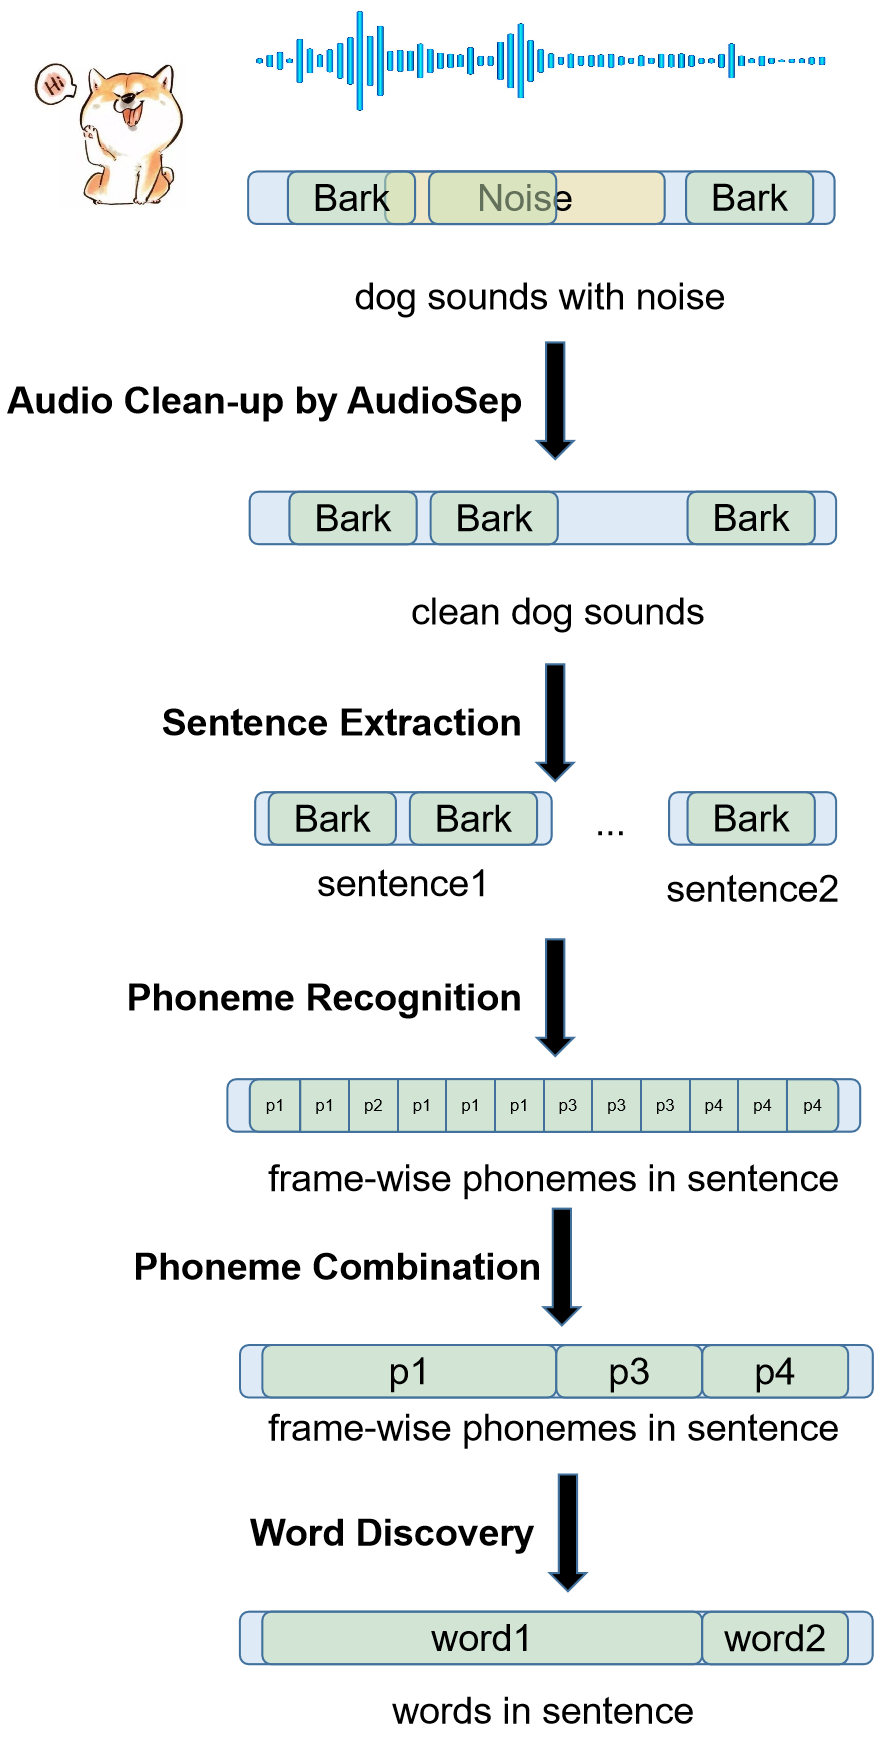
\includegraphics{workflow.png}}
    \caption{Full pipeline from data processing to word discovery.
%     \KZ{Change of the wordings in the fig to 
% ``Audio Clean-up by AudioSep'', ``Sentence Extraction'', ``Phoneme Recognition''. ``phonemes in sentence'' $\rightarrow$ ``frame-wise phonemes in sentence''}
}
    \label{fig:Workflow}
\end{figure}

\subsection{Audio Clean-up by AudioSep}

A mixture of dog sounds and noises will inevitably occur due to the use of videos from public social media. These noises can be background music edited in by the video uploader, human speeches, toy noises, etc. We expect a cleaner dataset, so we need to separate dog sounds from all mixed audios. In this work, we use AudioSep~\citep{liu2023separate}
% \MY{add a ~ before cite to insert space}
, a foundation model for open-domain audio source separation with natural language queries. The AudioSep is pre-trained on large-scale multimodal datasets, including AudioSet~\citep{gemmeke2017audio} dataset, VGGSound~\citep{chen2020vggsound} dataset, AudioCaps~\citep{kim2019audiocaps} dataset, etc. We apply AudioSep, using ``Dog'' as the input text query, to separate dog sounds from all audio. If it contains long audios that prevent AudioSep from running, you can start by cutting shorter audio clips with low-threshold~(less than 0.05) PANNs.
% \MY{Model accuracy should be reported and show that such separation will not greatly impact sound quality.}

To verify the effectiveness of AudioSep and to confirm that it did not have a significant impact on sound quality, we manually labeled 1467 seconds~(1137 seconds for train and 330 seconds for test) audios of dog barking to fine-tune the PANNs~\citep{kong2020panns}. The result~(\tabref{tab:audioSep_res}) shows that AudioSep can effectively reduce noise interference without significantly impacting the quality of dog sounds.

\begin{table}[h]
\centering
\begin{tabular}{lcc}
\hline
\textbf{Train Data} & \textbf{Test Data} & \textbf{F1 Score}\\
\hline
~~~~~~~~~- & - & 0.6916 \\
\hline
~~~~~~~~~\Checkmark{} & - & 0.6797 \\
\hline
~~~~~~~~~- & \Checkmark{} & \pmb{0.7755} \\
\hline
~~~~~~~~~\Checkmark{} & \Checkmark{} & 0.7709 \\
\hline
\end{tabular}
\caption{The result of PANNs. Those with a check mark are using AudioSep.}
\label{tab:audioSep_res}
\end{table}

\subsection{Sentence Extracting}
After the separation of dog sounds, the 
% \MY{how many audio clips are retained after audiosep?} \XY{I didn't write what I was coarsely screening the audio for, so do I not need to write the counts?}
audio will contain mostly barking, silence, and a small amount of noise that can't be separated. To focus on the part of dog sounds, we need to eliminate as much interference as possible from remaining silences and noises. To extract the part of dog sounds, we use a similar approach to \citet{huang2023transcribing}. We first apply PANNs~\citep{kong2020panns} trained on the large-scale AudioSet dataset to extract clips of dog sounds. Then, consecutive clips less than one second apart combine to form a dog ``sentence''. With AudioSep, we can get more and cleaner sentences than \citet{huang2023transcribing}.

To further eliminate noise, we use PANNs for audio tagging. Sentences that meet one of the following conditions will be filtered: (1) ``Dog'' label score less than 0.1. (2) Presence of labels not related to the dog with a score greater than 0.1.

\subsection{Phoneme Recognition}

Dog language is unfamiliar territory for humans. The lexicon, length, and other information of dog sound units are unknown, making it can not easily delineate sound units in a dog sentence in the same way that we delineate words in a human sentence. Directly using a priori knowledge of human language or the way to split human language units like \citet{huang2023transcribing} to understand dog language may be inapplicable. Self-supervised approaches for speech representation learning may be a more appropriate method for discovering the sound units of dog language. In this work, we use HuBERT, a self-supervised approach that learns a combined acoustic and language model over continuous inputs, to understand dog sound units. In \citeposs{hagiwara2023aves} work, Hubert has demonstrated a good ability to represent animal vocalization. So we use dog ``sentences'' to pre-train HuBERT. 
% Pretraining details can be found in Appendix~\ref{sec:appendix_a}.
% \MY{briefly introduce how Hubert is trained? that it contains two-step xxx. }

For HuBERT Pretraining, we used 54 clusters at the first stage and 100 clusters at the second stage, a learning rate of 0.0001, and 100k training steps at the first stage and 109k training steps at the second stage. Then we used features, which are from the 12th transformer layer of the second-stage model, to train a K-Means model with 50 clusters. The clusters are determined based on the sum of distances from each sample to its cluster center for different clusters (\figref{fig:clusters}).

\begin{figure}[h]
    \centering
    \scalebox{0.35}{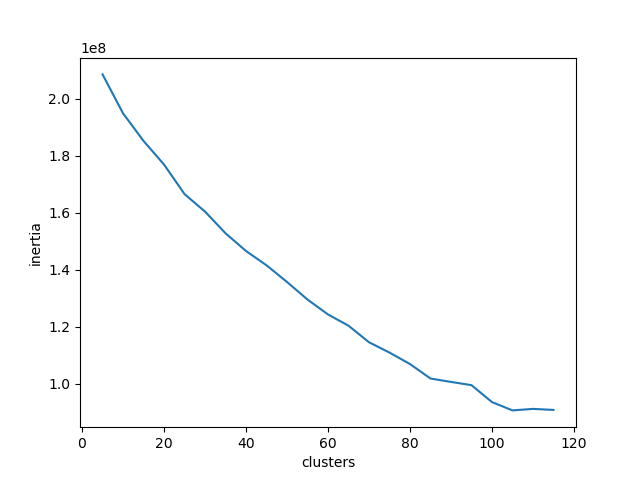
\includegraphics{clusters.png}}
    \caption{Inertia under different clusters. 50 is a suitable clusters. This is the basis for our choice of 50 clusters in the third K-Means model. The same method was used for the others.}
    \label{fig:clusters}
\end{figure}

\subsection{Phoneme Combination}
% \MY{Why selecting 50 as the K for clustering is something you need to justify. There are many details missing. You can add a training detail subsection in experiments, so that you concentrate on the method here and leave dataset specific details in the next section.}
After K-means clustering the features extracted from the approximately 20ms audio frames using HuBERT, we obtained a transcript with labels for each dog sound sentence. However, interestingly, the duration of a phoneme is often longer than 20ms. With the help of the excellent context recognition ability of the Transformer-based model, a large number of labels appear continuously in the transcript. After observing it, we found that there are still some noise segments in the transcript, such as a transcript containing the sequence: $[27, 27, 27, 5, 27, 27]$. After manual review of the original video, we found that the segment contains some faint noise. In order to obtain a purer transcript, we designed a phoneme combination algorithm.
% \MY{Training details should be reported for the two-step hubert pretraining, on what GPU, for how many epochs, optimizer, learning rate etc.}



% \begin{algorithm}
% \caption{An algorithm with caption}\label{alg:cap}
% \begin{algorithmic}
% \Require $n \geq 0$
% \Ensure $y = x^n$
% \State $y \gets 1$
% \State $X \gets x$
% \State $N \gets n$
% \For{\texttt{i in abc}}
% \EndFor
% \While{$N \neq 0$}
% \If{$N$ is even}
%     \State $X \gets X \times X$
%     \State $N \gets \frac{N}{2}$  \Comment{This is a comment}
% \ElsIf{$N$ is odd}
%     \State $y \gets y \times X$
%     \State $N \gets N - 1$
% \EndIf
% \EndWhile
% \end{algorithmic}
% \end{algorithm}

The algorithm uses double pointers to probe whether there are segments with the same label on both sides of the label. tolerance refers to the maximum length that can be assimilated by the labels on both sides. For example, when $tolerance=1$, the transcript segment $[a, a, b, b, a, a]$ cannot be optimized to $[a, a, a, a, a, a]$. After global phone combination optimization, we obtain the mean and standard deviation of the length of each phoneme.

\subsection{Word Discovery}

Once we obtained accurate labels for dog vocalization phonemes, we explored how to determine the ``word'' of a dog based on the current transcription.

\subsubsection{Enumeration}

To obtain a accurate ``vocabulary'', our first step is to list all possible words using the N-gram algorithm, which becomes the candidate vocabulary.
% \SN{It's quite easy, I think we can delete it}
\begin{algorithm}
\caption{Enumeration Algorithm}\label{alg:cap}
\begin{algorithmic}
\Require{$S \gets [s_1, s_2, s_3, ...]$}
\Require{$n$}
\Ensure{$ngrams$}
\State $ngrams \gets [ ]$
\State $i \gets 0$
\For{\texttt{seq in S}}
\State $l \gets len(seq)$
\State $i \gets 0$
\While{$i \leq l - n + 1$}
\State $ngram\gets seq[i:i+n]$
\State $i \gets i+1$
\State $ngrams$.append($ngram$)
\EndWhile
\EndFor
\end{algorithmic}
\end{algorithm}

\subsubsection{Scoring}

We believe that a word must satisfy the condition that it appears frequently enough in the transcription information to indicate its repeatability, and at the same time, we must ensure that the word is uttered by more than one dog to determine its universality. To this end, we designed a popularity score, the formula is as follows
$$Ps(gram^n_i) = f(gram^n_i) * \delta(gram^n_i)$$
, where $Ps(\cdot)$ is the popularity score function, $f(\cdot)$ is a function to calculate the frequency of this gram, $\delta(\cdot)$ is a function to calculate the diversity of this word, $gram^n_i$ is a unique n-gram, $n$ is the number of frames, $i$ indicates the $i_{th}$ unique ngram. The formula of $f$ and $\delta$ is as follows: 
\begin{eqnarray*}
f(gram^n_i) &=& \frac{\left | gram^n_i\right |}{\sum_{i}\left |gram^n_i\right |)}\\
\delta(gram^n_i) &=& \left |\{x\in D:x\ contains\ gram^n_i\}\right|,
\end{eqnarray*}
where $D$ is a set of different dogs in training dataset, $\left |\cdot \right |$ means to get the number of a set. 
The higher the popularity score of an ngram, the stronger the universality of the ngram, and its sound is uttered more times by more dogs.

\subsubsection{Filtering}

Once we have obtained the popularity score of all ngrams, the next question is how to filter them into the vocabulary. The first condition for an ngram to be called a ``word'' is its completeness. Inevitably, our ngrams with high popularity scores must contain incomplete ``words'', which are often part of a longer ngram. However, if we do not limit the selection of longer ngrams, our ``words'' will change from a single word to 2 or even a sentence. However, setting a threshold for the popularity score can help us avoid this problem. 

To this end, we set a hyperparameter \textbf{threshold} to ensure that the popularity score of ngrams included in the vocabulary is large enough, and start from the longest ngram and make sure that all words shorter than the ngram will not be part of the selected ngram. This ensures that the words in the vocabulary have complete attributes as much as possible. The selection of this hyperparameter can be done through recall, which will be discussed in \secref{sec:exp}.
